\textbf{Pregunta 7}
Let $P$ be a set of $n$ points in the plane. The staircase of $P$ is the set of all points
in the plane that have at least one point in $P$ both above and to the right.
\begin{center}
    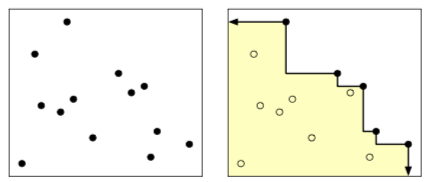
\includegraphics[scale=0.5]{escalera1}
\end{center}

\begin{enumerate}
\item Describe an algorithm to compute the staircase of a set of $n$ points in $O(n \log n)$ time.
      \newline
      
      A continuación exhibimos un algoritmo que soluciona el problema dado
      \begin{enumerate}
      \item Ordenar nuestra nube de puntos. Esto nos toma $\mathcal{O}(n \log n)$.
      \item Esta parte es un poco parecida a encontrar la envolvente convexa de una
            nube de puntos. Así,
           \begin{enumerate}
           \item Encontrar el punto $p_1$ más alto (con mayor valor respecto de $Y$). Esto nos toma $\mathcal{O}(\log n)$
                 realizando una búsqueda binaria.
           \item Encontrar el punto $p_2$ a la derecha de $p_1$ y que además sea el más alto del subconjunto de puntos
           menos $p_1$. Digamos que inicialmente $p_1$ era nuestro elemento pivotante, en este punto cambiemos nuestro
           pivote por $p_2$.
           \item Repetimos para $p_2$ y de manera iterativa, hasta no encontrar algún elemento a la derecha. 
           \end{enumerate}
           Todo esto se hace en a lo más $\mathcal{O}(n \log n)$.
      \item Ahora que tenemos una selección que formará nuestra escalera podemos construir la misma de la siguiente manera:
            \begin{enumerate}
            \item Notemos que el paso anterior nos da los puntos en el orden que deben encontrarse en nuestra escalera (descendiente).
            \item Tomemos dos puntos de nuestra selección, los más cercanos en ella (equivale a tomar los consecutivos si se guardan
            en una lista) y proyectemos al primero de manera vértical y al segundo de manera horizontal (recordar que el primer
            elemento es el más ``alto'' de todos), el corte de las proyecciones lo podemos llamar ``vértice artificial'' y así
            podemos incluir la estructura en nuestra escalera. Es decir, unimos los vértice por medio del corte formado en
            el vértice artificial.
            \item Repetimos hasta acabar con los vértices de la selección.
            \end{enumerate}
            Lo anterior nos toma a lo más $\mathcal{O}(n)$.
      \end{enumerate}
      Finalmente, devolvemos la construcción hecha en $(c)$.\newline

      \textit{Análisis de complejidad.} Podemos notar que nuestra complejidad en tiempo está contenida en
      \[\mathcal{O}(n\log n) + \mathcal{O}(n\log n) + \mathcal{O}(n) = \mathcal{O}(n\log n).\]
\item Describe and analyze a data structure that stores the staircase of a set of points, and an
  algorithm ABOVE? $(x, y)$ that returns \textsc{true} if the point $(x, y)$ is above the staircase,
  or \textsc{fals} otherwise. Your data structure should use $O(n)$ space, and your ABOVE? algorithm
  should run in $O(log n)$ time.
\end{enumerate}

\begin{center}
    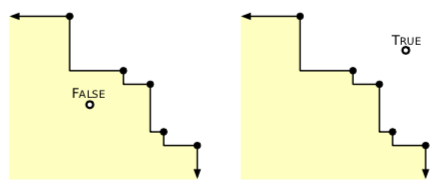
\includegraphics[scale=0.5]{escalera2}
\end{center}


  Cómo entrada tenemos nuestra escalera que es a lo más de orde $\mathcal{O}(n)$, por tanto es suficiente
  con almacenar esta para responder nuestra pregunta. ¿Cómo lo hacemos?
  \begin{itemize}
  \item La idea será similar a los árboles de segmentos.
  \item Guardamos cada segmento en un nodo.
  \item Para construir este árbol basta dividir con un ``rayo'' nuestra escalera, así vamos equilibrando nuestro árbol
  (de hecho es exactamente igual a un árbol de segmentos).
  \item \textbf{Consultar.} Basta verificar si nuestro segmento es horizontal o vértical.
  \begin{itemize}
  \item Si es horizontal basta comparar el punto $x$\footnote{Punto a comparar.} con un extremo del segmento, si
  $x$ es mayor, entonces verificamos si queda a la izquierda o derecha de nuestra escalera. Si sí regresamos TRUE, FALSE en otro caso.
  \item Si es vértical basta verificar si $x$ es mayor al extremo superior del segmento, si sí entonces verificamos si se
  encuentra a la izquierda o derecha de la escalera. Si sí, entonces devolvemos TRUE. FALSE en otro caso.
  \end{itemize}    
  \end{itemize}

Cómo basta con bajar por nuestro árbol y es un árbol binario balanceado, entonces garantizamos que la consulta se realiza en $\mathcal{O}(\log n)$.
